% !TeX encoding = UTF-8
% !TeX spellcheck = en_US
\documentclass[a4paper,14pt]{extarticle} %размер бумаги устанавливаем А4, шрифт 14пунктов
\usepackage{amssymb,amsfonts,amsmath,mathtext,cite,enumerate,float} %подключаем нужные пакеты расширений
\usepackage[T2A, T1]{fontenc}
\usepackage{cmap}
\usepackage[utf8]{inputenc}%включаем свою кодировку: koi8-r или utf8 в UNIX, cp1251 в Windows
\usepackage[english, russian]{babel}%используем русский и английский языки с переносами

\usepackage{graphicx} %хотим вставлять в диплом рисунки?
\graphicspath{{images/}}%путь к рисункам

%{tikz}
\usepackage{pgfplots}

\usepackage{listings}
\lstset{
	frame=single,
	breaklines=true
}
\lstset{language=C++,
	basicstyle=\ttfamily,
	keywordstyle=\color{blue}\ttfamily,
	stringstyle=\color{red}\ttfamily,
	commentstyle=\color{green}\ttfamily,
	morecomment=[l][\color{magenta}]{\#}
}

\usepackage[colorlinks=false,pdfborder={0 0 0}]{hyperref} %использование гиперссылок, colorlinks - цвет текста ссылки, pdfborder - окантовка. 

%шрифт Times New Roman
%\usepackage{fontspec}
%\setmainfont{Times New Roman}
%\setallmainfonts{Times New Roman}

\usepackage{titlesec}
\titleformat{\section}[block]
{\filcenter\large}
{\thesection}
{1em}{\MakeUppercase}
\titlespacing*{\section}{0pt}{-30pt}{*4}

\makeatletter
%\renewcommand{\@biblabel}[1]{#1.} % Заменяем библиографию с квадратных скобок на точку:
\makeatother


\usepackage{geometry} % Меняем поля страницы
\geometry{left=3cm}% левое поле
\geometry{right=15mm}% правое поле
\geometry{top=2cm}% верхнее поле
\geometry{bottom=2cm}% нижнее поле
\linespread{1.5}

\usepackage{indentfirst} % отделять первую строку раздела абзацным отступом
\setlength\parindent{5ex}

%links
\usepackage{url}

\usepackage[tableposition=top,singlelinecheck=false, justification=centering]{caption}
\usepackage{subcaption}

%  маркированные списки
\renewcommand{\labelitemi}{--}
\renewcommand{\labelitemii}{--}
%  нумерованные списки
\renewcommand{\labelenumi}{\asbuk{enumi})}
\renewcommand{\labelenumii}{\arabic{enumii})}

% номер сноски со скобкой
\renewcommand*{\thefootnote}{\arabic{footnote})}
\renewcommand{\footnoterule}{%
	\kern -3pt
	\hrule width 40mm height .4pt
	\kern 2.6pt
}

%иллюстрации и таблицы
\DeclareCaptionLabelFormat{gostfigure}{Рисунок #2}
\DeclareCaptionLabelFormat{gosttable}{Таблица #2}
\DeclareCaptionLabelSeparator{gost}{~---~}
\captionsetup{labelsep=gost}
\captionsetup*[figure]{labelformat=gostfigure}
\captionsetup*[table]{labelformat=gosttable}
\renewcommand{\thesubfigure}{\asbuk{subfigure}}


%\renewcommand{\rmdefault}{ftm}
\renewcommand{\figurename}{Рисунок} % Рис -> Рисунок
%\usepackage[labelsep=period,labelfont=bf,figurename={Рисунок},figurewithin=none]{caption}
\renewcommand{\theenumi}{\arabic{enumi}}% Меняем везде перечисления на цифра.цифра
\renewcommand{\labelenumi}{\arabic{enumi}}% Меняем везде перечисления на цифра.цифра
\renewcommand{\theenumii}{.\arabic{enumii}}% Меняем везде перечисления на цифра.цифра
\renewcommand{\labelenumii}{\arabic{enumi}.\arabic{enumii}.}% Меняем везде перечисления на цифра.цифра
\renewcommand{\theenumiii}{.\arabic{enumiii}}% Меняем везде перечисления на цифра.цифра
\renewcommand{\labelenumiii}{\arabic{enumi}.\arabic{enumii}.\arabic{enumiii}.}% Меняем везде перечисления на цифра.цифра

\usepackage{tocloft}
\renewcommand{\cftsecleader}{\cftdotfill{\cftdotsep}}
%\renewcommand{\cfttoctitlefont}{\Large\filcenter}

%\setcounter{page}{2} %нумерация страниц с 3
%\addto\captionsrussian{\renewcommand\contentsname{СОДЕРЖАНИЕ}}
%\addto\captionsrussian{\renewcommand\refname{СПИСОК ИСПОЛЬЗОВАНЫХ ИСТОЧНИКОВ}}



\begin{document}
	% !TeX spellcheck = ru_RU
% !TeX encoding = UTF-8
\subsection{АБГШ}
\label{sec:awgn}

Аддитивный Белый Гауссовский Шум (АБГШ) является видом мешающего воздействия в канале связи или других процессах. Определяется данный вид шума как гауссовский случайный процесс $n(t )$ с нулевым средним и спектральной плотностью мощности $S_n( f ) = N_0 / 2$. АБГШ является наиболее распространённым видом шума, используемым для расчёта и моделирования систем связи. Термин «аддитивный» означает, что данный вид шума суммируется с исходным сигналом и статистически не зависим от сигнала.

Дисперсия АБГШ может быть вычислена как $\sigma^2 = \int_{-\infty}^{\infty}S_n(f)df$. Так как АБГШ существует во всей полосе частот $-\infty < f < \infty$, то $\sigma^2 = \infty$. В реальности такого не может существовать, т.к. бесконечно большой мощности не может быть. Шум не может существовать без сигнала, таким образом, ширина полосы частот шума зависит от ширины полосы частот исходного сигнала. 
	% !TeX spellcheck = ru_RU
% !TeX encoding = UTF-8
\section{Теоретическая вероятность в двоичном канале с аддитивным белым гуассовским шумом}

Рассмотрим систему передачи двоичных сигналов $0$ и $1$. Вероятность ошибки в такой системе определяется по следующей формуле:

\begin{equation}
	P_e = \sum_{i=0}^{1}P_e(i)P_i = P_e(0)P_0 + P_e(1)P_1,
\end{equation}

где $P_e(i)$ -- условная вероятность ошибки при передаче $i$-го сигнала, $P_i$ -- вероятность передачи $i$-го сигнала. Рассмотрим простую систему с одинаковыми вероятностями передачи сигналов. Таким образом, можно рассчитать вероятность ошибки для одного символа, эта же вероятность будет являться вероятностью ошибки для всей системы. Вероятность ошибки будем рассчитывать по максимальному правдоподобию:
\begin{equation}
	\label{form:pe_1}
	P_e(0) = Pr[d^2(r,s_0) > d^2(r,s_1) \mid 0] = Pr[ || r - s_0||^2 > ||r - s_1||^2 \mid 0] ,
\end{equation}

где $r$ -- принятый сигнал, $s_i$ -- переданный $i$-ый сигнал. При этом нужно учесть, что $r = s_i + n$, где $n$ -- АБГШ, который описан в разделе \ref{sec:awgn}. Тогда формула (\ref{form:pe_1}) приобретает вид:
\begin{equation}
	P_e(0) = Pr[||n||^2 > ||s_0 - s_1 + n||^2] = Pr[||n||^2 - ||s_0 - s_1 + n||^2 > 0].
\end{equation}
Выражение $||n||^2 - ||s_0 - s_1 + n||^2$ при раскрытии скобок преобразуется в 
\begin{equation}
\begin{split}
	||n||^2 - ||s_0 - s_1 + n||^2 = ||n||^2 - ||s_0 - s_1||^2 - 2\sum_{j=1}^{D}(s_{0j} - s_{1j}) n_j\\ - ||n||^2 = 
	 - ||s_0 - s_1||^2 - 2\sum_{j=1}^{D}(s_{0j} - s_{1j}) n_j.
\end{split}
\end{equation}
Произведем замену переменных $\Delta^2 =-2||s_0 - s_1||^2$ и $\epsilon =  -2\sum_{j=1}^{D}(s_{0j} - s_{1j}) n_j$, тогда 
\begin{equation}
	P_e(0) = Pr[\epsilon > \Delta^2].
\end{equation}
Стоит отметить, что $\epsilon$ является случайной гуассовской величиной, т.к. является линейной комбинацией разности сигналов и АБГШ. Принимая в расчет, что математическое ожидание АБГШ равно $0$, то $\bar{\epsilon} = 0$, а дисперсия $D[\epsilon] = 2N_0\Delta^2$.

Для дальнейших расчетов необходимо ввести Q-функцию, которая позволяет найти вероятность превышения некоторого порога $A$ гауссовской случайной величиной $x$ с параметрами $(m,\sigma^2)$:

\begin{equation}
	Pr[x > A] = Q(\frac{A - m}{\sigma}).
\end{equation}

Q-функция определяется следующей формулой:

\begin{equation}
	Q(x) = \int_{x}^{\infty}{\frac{1}{\sqrt{2\pi}}}e^{-z^2 / 2}dz
\end{equation} 

С учетом вышесказанного:
\begin{equation}
	P_e(0) = Q(\frac{\Delta^2}{\sqrt{\Delta^22N_0}}) = Q(\frac{\Delta}{\sqrt{2N_0}}).
\end{equation}

Так как $P_e(0)$ = $P_e(1)$, то
\begin{equation}
	P_e = Q(\frac{\Delta}{\sqrt{2N_0}}).
\end{equation}

Таким образом, вероятность ошибки дыоичных сигналов в канале с АБГШ зависит от величины евклидова расстояния между сигналами и интенсивности шума. При этом стоит учесть, что вид сигналов значения не имеет.
	% !TeX spellcheck = ru_RU
% !TeX encoding = UTF-8
\subsection{Почему зону покрытия абонентской станции изображают шестиугольником}

%шестиугольником можно покрыть пространство без дыр, так же, как и квадратом или треугольником
%шестиугольник ближе к кругу, ежели квадрат или треугольник
%диаграммы воронова


На заре развития беспроводной связи перед исследователями и инженерами-связистами встала задача, как изображать границы принимаемого сигнала Абонентскими Станциями (АС). По своей природе АС имеют круговую диаграмму направленности. Но если изображать границы сигнала кругами, то карта АС становится перегруженной. Из геометрии известно, что существует три типа многоугольников, которыми можно заполнить пространство: треугольники, квадраты и шестиугольники. Из этих трех фигур шестиугольник ближе всего к кругу, которым описывается граница области покрытия АС. 

При этом стоит отметить, что шестиугольники удобны только в случае АС с одинаковой мощностью и зоной покрытия, расположенные по сетке с одинаковым шагом. Когда на области существуют разные виды АС, которые удалены друг от друга на разное расстояние, используют диаграммы Вороного. 

\subsubsection{Диаграмы Вороного}

Диаграммы Вороного используются во многих областях жизнедеятельности человека, в том числе телекоммуникациях. Для начала введем понятия нужных для понимания геометрических объектов:

\begin{itemize}
	\item Простой многоугольник -- это многоугольник без самопересечений. Мы будем рассматривать только простые многоугольники.
	\item Невыпуклый многоугольник -- это многоугольник, в котором есть такие две вершины, что через них проводится прямая, пересекающая данный многоугольник где-либо ещё, кроме ребра, соединяющего эти вершины (рисунок \ref{fig:mnogoug}), 
	\item Выпуклый многоугольник -- это многоугольник, у которого продолжения сторон не пересекают других его сторон рисунок \ref{fig:mnogoug}).
\end{itemize}

\begin{figure}[h]
	\centering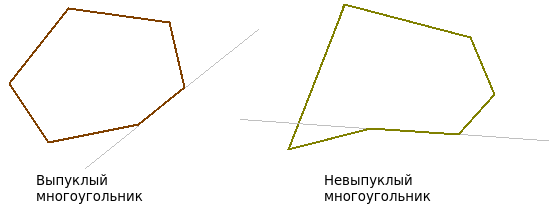
\includegraphics[width=0.7\linewidth]{mnogoug}
	\caption{Примеры выпуклого и невыпуклого многоугольников}
	\label{fig:mnogoug}
\end{figure}

Именно из выпуклых многоугольников и будет состоять диаграмма, так как они являются ничем иным, как пересечением полуплоскостей, которые являются выпуклыми фигурами.

Диаграмма состоит из локусов -- областей, в которых присутствуют все точки, которые находятся ближе к данной точке, чем ко всем остальным. В диаграмме Вороного локусы являются выпуклыми многоугольниками.

По определению локус строится следующим образом: пусть дано множество из $n$ точек, для которого мы строим диаграмму. Возьмём конкретную точку $p$, для которой строим локус, и ещё одну точку из данного нам множества $q$ не равную $p$. Проведём отрезок, соединяющий эти две точки, и проведём прямую, которая будет являться серединным перпендикуляром данного отрезка. Эта прямая делит плоскость на две полуплоскости. В одной лежит точка $p$, в другой лежит точка $q$. В данном случае локусами этих двух точек являются полученные полуплоскости. То есть для того, чтобы построить локус точки $p$, нужно получить пересечение всех таких полуплоскостей. То есть на месте $q$ должны быть все точки данного множества, кроме $p$.

\begin{figure}[h]
	\centering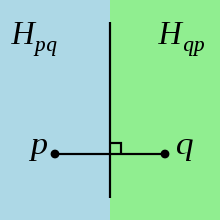
\includegraphics[width=0.3\linewidth]{polupl}
	\caption{Пример полуплоскостей}
	\label{fig:polupl}
\end{figure}

Точку, для которой строится локус, называют сайтом (site). На рисунке \ref{fig:sites} локусы помечены разными цветами.

\begin{figure}[h]
	\centering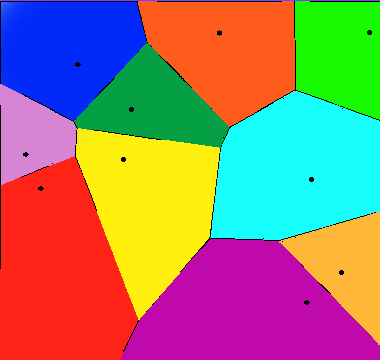
\includegraphics[width=0.4\linewidth]{sites}
	\caption{Сайты в диаграмме Вороного}
	\label{fig:sites}
\end{figure}

Алгоритмы построения диаграммы строят локусы для всех точек из заданного набора. Локусы в данной задаче также называют многоугольниками Вороного или ячейками Вороного. 

Наконец, сформулируем определение диаграммы Вороного $n$ точек на плоскости -- это разбиение плоскости, состоящее из $n$ локусов. 

\subsubsection{Алгоритм построения диаграммы Вороного}

Основная идея алгоритма в том, чтобы пересекать не полуплоскости, а именно серединные перпендикуляры отрезков, так как это проще, соединяющих данную точку со всеми другими точками. То есть, следуя определению ячейки Вороного, мы будем строить локус для точки $p$ следующим образом:

\begin{enumerate}
	\item Получаем $n-1$ прямую (серединные перпендикуляры), так как мы провели серединные перпендикуляры всех отрезков, соединяющих данную точку $p$ с остальными;
	\item Пересекаем попарно все прямые, получаем $O(n^2)$ точек пересечения (потому что каждая прямая может пересечь все другие, в «худшем случае»);
	\item Проверяем все эти $O(n^2)$ точек на принадлежность каждой из $n-1$ полуплоскостей, то есть получаем уже асимптотику $O(n^3)$. Соответственно те точки, которые принадлежат всем полуплоскостям, и будут вершинами ячейки Вороного точки $p$;
\end{enumerate}

Проделываем первые три шага для всех $n$ точек, получаем итоговую асимптотику $O(n^4)$.

%    \subsection{Защитный интервал в сетях LTE}
Рассмотрим систему, изображенную на рисунке~\ref{fig:vol_mobile_cell}.
\begin{figure}[H]
    \centering
    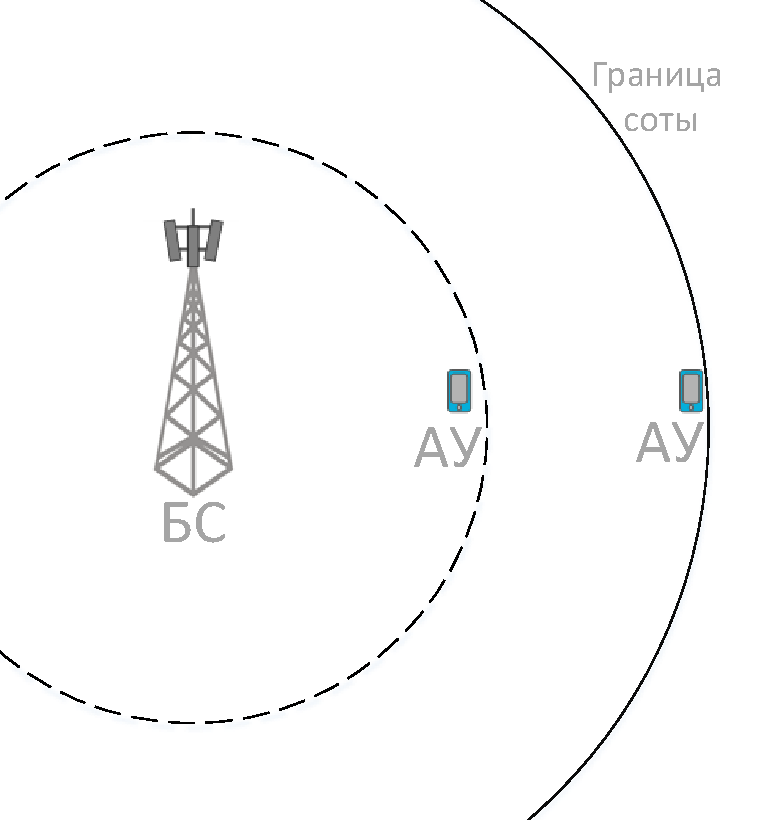
\includegraphics[width=0.5\textwidth]{img/vol_mobile_cell}
    \caption{Мобильная сота с двумя абонентами}
    \label{fig:vol_mobile_cell}
\end{figure}

Данная система состоит из базовой станции (БС) и двух абонентских устройств (АУ), один из которых
расположен непосредственно у базовой станции, второй --- на границе соты. Ни АУ, ни БС не могут знать
точное время появления данных в пределах установленного окна, так как информация передается с
некоторой задержкой. Если задержка одного из передаваемых сообщений окажется слишком большой, то
данное сообщение выйдет за границы собственного окна. Это может привести к наложению одного сообщения
на другое --- к интерференции, в результате которой принятые сообщения будет невозможно корректно
обработать. Подобный случай приведен на рисунке~\ref{fig:vol_interf}
\begin{figure}[H]
    \centering
    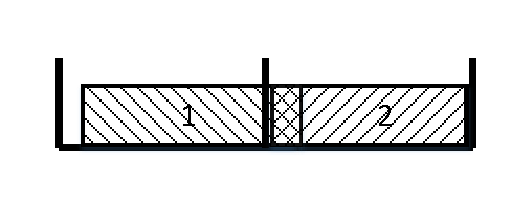
\includegraphics[width=0.5\textwidth]{img/vol_interf}
    \caption{Интерференция двух сообщений}
    \label{fig:vol_interf}
\end{figure}
Для устранения подобного эффекта вводится специальный параметр --- защитный интервал.
При использовании данного параметра время передачи сообщения сокращается. Освободившийся интервал
времени (защитный интервал) делится на две части: циклический префикс (ЦП) и защитное время (ЗВ).
ЦП является избыточной информацией и представляет собой повторение конца сообщения.
Он необходим для корректной обработки в тех случаях, когда сообщение вышло за границы
собственного окна. ЗВ необходим для того, чтобы снизить влияние задержки на передачу сообщений
абонентам, находящимся на больших расстояниях от базовой станции. Пример такого случая
приведен на рисунке~\ref{fig:vol_CP}. 
\begin{figure}[H]
    \centering
    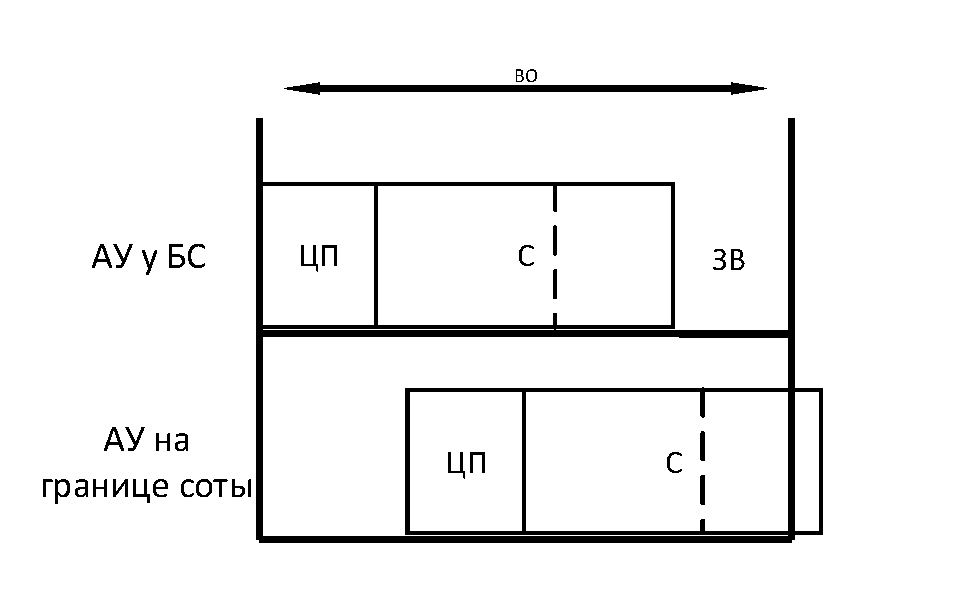
\includegraphics[width=0.75\textwidth]{img/vol_CP}
    \caption{Использование циклического префикса}
    \label{fig:vol_CP}
\end{figure}

Ошибки синхронизации, различные задержки при передаче сообщений приводят к интерференции.
Использование ЦП и ЗВ позволяет сократить возможность возникновения подобного явления.

Выбор размера ЦП и ЗВ во многом зависит от характера местности и размера соты. Для определения
влияния размера соты на значение ЦП рассмотрим рисунок~\ref{fig:vol_calc_CP}.
\begin{figure}[H]
    \centering
    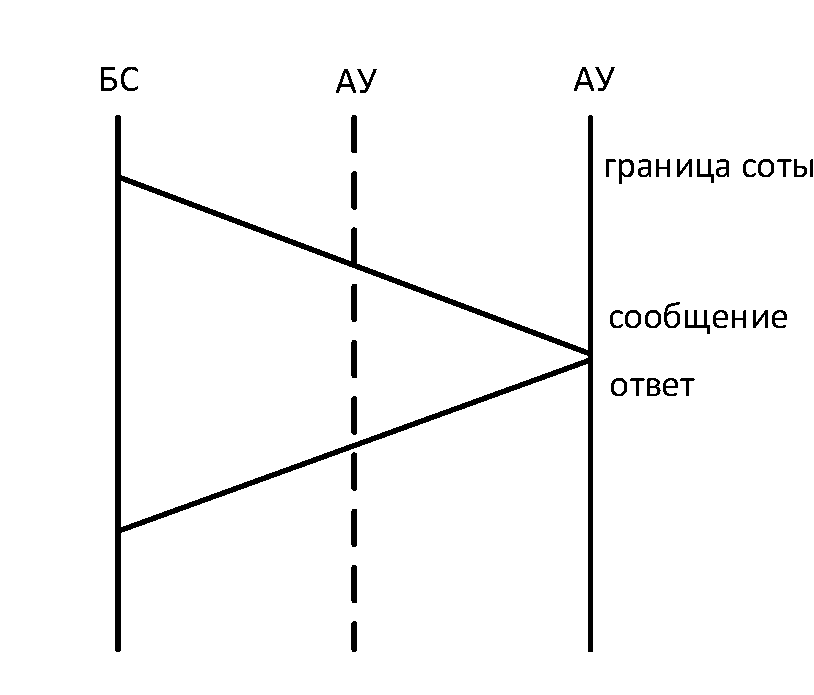
\includegraphics[width=0.5\textwidth]{img/vol_calc_CP}
    \caption{Передача сообщения от БС к АУ на границе соты}
    \label{fig:vol_calc_CP}
\end{figure}

Известно, что радиосигнал распространяется со скоростью примерно равной скорости света \(c = 3 \cdot
10^{8}\) м/с. Таким образом, время распространения сигнала от БС до дальнего АУ равно
\(T = \dfrac{Cell Size}{c}\). Но для завершения передачи БС должна получить ответ от АУ.
Время распространения ответа равно времени распространения сообщения \(T = \dfrac{2 \cdot Cell
Size}{c}\). Таким образом, через время, равное \(Т\), сообщение поступит на АУ, а спустя небольшую
задержку поступят переотраженные сигналы \((d)\).
Отсюда можно сделать вывод, что размер защитного интервала должен быть равен времени распространения
сигнала. В итоге размер циклического префикса равен \[T_{CP} = T = \dfrac{2 \cdot Cell Size}{c} + d\].


%    \subsection{Дискретное преобразование Фурье}
Дискретное преобразование Фурье (ДПФ) --- инструмент спектрального анализа сигналов. ДПФ позволяет сопоставить сигналу во временной области эквивалентное представление в частотной области.
Данное преобразование ставит в соответствие \(N\) отсчетам сигнала \(s(n), n = 0, 1 \dots N-1,  N\) отсчетов комплексного \(S_d(k), k = 0 \dots N-1 \).

Формула преобразования имеет следующий вид:
\begin{equation}
    S(k) = \sum_{n=0}^{N-1} s(n) \cdot e^{-j \cdot \dfrac{2\pi}{N} \cdot n \cdot k}, k = 0 \dots N-1
\end{equation}

Согласно формуле Эйлера \(e^{jx} = \cos(x) + j\sin(x)\) преобразование Фурье может быть представлено в следующем виде:
\begin{equation} \label{eq:DFT_cos}
    S(k) = \sum_{n=0}^{N-1} s(n) \cdot (\cos(\dfrac{2\pi}{N} \cdot n \cdot k) - j \sin(\dfrac{2\pi}{N} \cdot n \cdot k))
\end{equation}

В качестве примера рассмотрим вектор чисел размером \(N = 8 \)
\begin{equation*}
    s(n) = [0.5, 0.2, 0, 0, 0, 0, 0, 0]
\end{equation*}
Согласно формуле (\ref{eq:DFT_cos}) данный вектор поэлементно умножается на \(\cos\) и \(\sin\):
\begin{table}[H]
    \centering
    \begin{tabular}{c}
        k = 0: \(cos(0) - j \cdot sin(0)\); \\
        k = 1: \(cos(\dfrac{2\pi}{N} \cdot n) - j \cdot sin(\dfrac{2\pi}{N} \cdot n);\) \\
        k = 2: \(cos(\dfrac{2\pi}{N} \cdot 2 \cdot n) - j \cdot sin(\dfrac{2\pi}{N} \cdot 2 \cdot n);\)  \\
        k = 3: \(cos(\dfrac{2\pi}{N} \cdot 3 \cdot n) - j \cdot sin(\dfrac{2\pi}{N} \cdot 3 \cdot  n);\) \\
        k = 4: \(cos(\dfrac{2\pi}{N} \cdot 4 \cdot n) - j \cdot sin(\dfrac{2\pi}{N} \cdot 4 \cdot n);\)  \\
        k = 5: \(cos(\dfrac{2\pi}{N} \cdot 5 \cdot n) - j \cdot sin(\dfrac{2\pi}{N} \cdot 5 \cdot n);\) \\
        k = 6: \(cos(\dfrac{2\pi}{N} \cdot 6 \cdot n) - j \cdot sin(\dfrac{2\pi}{N} \cdot 6 \cdot n);\)  \\
        k = 7: \(cos(\dfrac{2\pi}{N} \cdot 7 \cdot n) - j \cdot sin(\dfrac{2\pi}{N} \cdot 7 \cdot n);\) \\
    \end{tabular}
\end{table}
В результате такого перемножения будет получен следующий вектор:
\begin{table}[H]
    \centering
    \begin{tabular}{ll}
        \(S(n) = [\) & 
        \(0.7 + j \cdot 0\); \\
        & \(0.6414 - j \cdot 0.1414\); \\
        & \(0.5 - j \cdot 0.2\); \\
        & \(0.3586 - j \cdot 0.1414\); \\
        & \(0.3 + j \cdot 0\); \\
        & \(0.3586 + j \cdot 0.1414\); \\
        & \(0.5 + j \cdot 0.2\); \\
        & \(0.6414 + j \cdot 0.1414]\); \\
    \end{tabular}
\end{table}
	%	\bibliographystyle{gost2008l}  %% стилевой файл для оформления по ГОСТу
	%	\bibliography{biblio}     %% имя библиографической базы (bib-файла) 
		\addcontentsline{toc}{subsection}{Список использованных источников}
\end{document}